% para impressão considerar a troca de oneside para twoside
\documentclass[a4paper, 12pt, openany, oneside, english, brazil, fleqn]{abntex2}
\usepackage[brazil]{babel}
\usepackage{enumerate}
\usepackage[utf8]{inputenc}
% \usepackage[latin1]{inputenc}
\usepackage[T1]{fontenc}
\DisemulatePackage{setspace}
\usepackage{setspace}
\usepackage{dsfont}
\usepackage{titlesec}
\usepackage{cmap}
\usepackage{lmodern}
\usepackage{amssymb,amsmath}
\usepackage{multirow}
\usepackage{color, graphicx}
\usepackage{colortbl}
\usepackage{soul}
\usepackage{xcolor}
\usepackage{url}
\usepackage{booktabs}
\usepackage{microtype} 			% para melhorias de justificação
% Sistema autor-data
\usepackage[alf]{abntex2cite}
\usepackage{indentfirst} % paragrafo na primeira linha escrita
% Pacote para o uso de algoritmos
\usepackage{pdflscape}
\usepackage[portuguese, ruled, linesnumbered, noline]{algorithm2e}
% \usepackage{comment}
\usepackage{geometry}
\geometry{ left=30mm, top=30mm, right=20mm, bottom=20mm }%considerando sempre frente
\setlength{\textfloatsep}{0pt}
\setlength{\mathindent}{0cm}
\setlength{\abovedisplayskip}{12pt}
\setlength{\belowdisplayskip}{12pt}
\usepackage[font=small,skip=0pt]{caption}
\setlength{\parskip}{12pt}
%\setlength{\belowcaptionskip}{12pt}
%\titleformat{\chapter}{\bfseries}{\chaptername}{\thechapter}{0pt}{\vskip 20pt\raggedright}% \titlespacing{<command>}{<left>}{<before-sep>}{<after-sep>}[<right>]
%\titlespacing*{\section}{0pt}{\baselineski}{\baselineskip}{0pt}%does not work with \chapter
\newcommand{\curso}[1]{\def\imprimircurso{#1}}
\newcommand{\dataDaAprovacao}[1]{\def\imprimirdatadaaprovacao{#1}}
\newcommand{\tituloEstrangeiro}[1]{\def\imprimirtituloestrangeiro{#1}}

\renewcommand{\imprimircapa}{%
  \begin{capa}
    \begin{center}

      % Cabeçalho (não deve ser modificado)
      % Contém o brasão da Universidade, além dos dados
      % relacionados à vinculação do aluno (Universidade, Centro, Departamento e Curso)
      \begin{figure}
        \begin{center}
          
\includegraphics[width=2.53cm, height=3.1cm]{imagens/brasao.png}
        \end{center}
      \end{figure}
        \begin{center}
            {\large \textsc{Universidade Federal do Rio Grande do Norte}}
            \vspace{-0.3cm}
        \end{center}	
        \begin{center}
            {\large \textsc{Instituto Metrópole Digital}}
            \vspace{-0.3cm}
        \end{center}
        \begin{center}
          {\large \textsc{Programa de Pós-Graduação em Inovação em Tecnologias Educacionais}}
        \end{center}

      \vspace{6cm}

      % Título do trabalho
      {\setlength{\baselineskip}
      {1.3\baselineskip}
      {\LARGE \textsc{\imprimirtitulo}}\par}

      \vspace{8cm}

      % Nome do aluno (autor)

      {\Large \textsc{\imprimirautor}}

      % Local da instituição onde o trabalho deve ser apresentado e ano de entrega do mesmo
      {\Large \imprimirlocal, \imprimirdata} 
    \end{center}
  \end{capa}

  % Solução para geração de páginas duplicadas, uma delas fica em branco
  \hypersetup{pageanchor=true}
}

% Conteudo padrao da Folha de Rosto
\makeatletter
\renewcommand{\folhaderostocontent} {
  \begin{center}

 \begin{figure}
        \begin{center}
          
\includegraphics[width=2.53cm, height=2.96cm]{imagens/brasao.png}
        \end{center}
      \end{figure}
      \begin{center}
            {\large \textsc{Universidade Federal do Rio Grande do Norte}}
            \vspace{-0.3cm}
        \end{center}
        \begin{center}
            {\large \textsc{Instituto Metrópole Digital}}
            \vspace{-0.3cm}
        \end{center}
        \begin{center}
          {\large \textsc{Programa de Pós-Graduação em Inovação em Tecnologias Educacionais}}
        \end{center}

	\vspace{3cm}

 	\begin{center}
      {\LARGE \textsc{\imprimirtitulo}}\par
    \end{center}
    
    \vspace{3cm}

    {\large \textsc{\imprimirautor}}
\SingleSpacing
    \abntex@ifnotempty{\imprimirpreambulo}{%
      \hspace{.45\textwidth}
      \begin{minipage}{.5\textwidth}
      \begin{OnehalfSpace}
          {\large \imprimirpreambulo}
      \end{OnehalfSpace}
      \end{minipage}%
    }%
\SingleSpacing
    {\Large\imprimirlocal}
    
    {\Large\imprimirdata}

  \end{center}
}
\makeatother

%% Redefinicao de instrucoes
\floatname{algorithm}{Algoritmo}
\renewcommand{\algorithmicrequire}{\textbf{Entrada:}}
\renewcommand{\algorithmicensure}{\textbf{Saída:}}
\renewcommand{\algorithmicend}{\textbf{fim}}
\renewcommand{\algorithmicif}{\textbf{se}}
\renewcommand{\algorithmicthen}{\textbf{então}}
\renewcommand{\algorithmicelse}{\textbf{senão}}
\renewcommand{\algorithmicfor}{\textbf{para}}
\renewcommand{\algorithmicforall}{\textbf{para todo}}
\renewcommand{\algorithmicdo}{\textbf{faça}}
\renewcommand{\algorithmicwhile}{\textbf{enquanto}}
\renewcommand{\algorithmicloop}{\textbf{loop}}
\renewcommand{\algorithmicrepeat}{\textbf{repetir}}
\renewcommand{\algorithmicuntil}{\textbf{até que}}
\renewcommand{\algorithmiccomment}[1]{\% #1}

% \listofalgorithms: comando que imprime a lista de algoritmos
\renewcommand{\listalgorithmname}{Lista de algoritmos}

% Redefinindo as cores dos links (pacote hyperref)
% O hyperref é incluso automaticamente pelo abntex2
\hypersetup{pageanchor=false,
              colorlinks=true,
              linkcolor=black,
              citecolor=black,
              urlcolor=blue}


% Redefinicao de alguns comandos do pacote algorithm2e
\SetKwBlock{Inicio}{in\'{i}cio}{fim}
\SetKwFor{Para}{para}{fa\c{c}a}{fim para}%
\SetKwFor{ParaCada}{para cada}{fa\c{c}a}{fim para}%
\SetKwIF{Se}{SenaoSe}{Senao}{se}{ent\~{a}o}{sen\~{a}o se}{sen\~{a}o}{fim se}%
\SetKwRepeat{Repita}{repita}{at\'{e}}%

% espaçamento entre linhas 1.5cm segundo ABNT, por padrão a classe antex2 já é 1.5.
% \OnehalfSpacing (padrão) or \DoubleSpace para mudar
% Recuo do parágrafo em 1.5cm
\setlength{\parindent}{1.5cm}

% Texto padrão fontes do capítulo em Latin Mordern Roman (lmodern), mesma fonte usada no texto
\renewcommand{\ABNTEXchapterfont}{\fontfamily{lmr}\fontseries{b}\selectfont}

% Dados pessoais
\autor{Nome do aluno}
\curso{Mestrado em Inovação em Tecnologias Educacionais}

% Dados do trabalho
\titulo{Título do Trabalho}
\tituloEstrangeiro{Título do trabalho (em língua estrangeira)}
\data{20XX}
%\palavraChaveUm{Palavra-chave01}
%\palavraChaveDois{Palavra-chave02}

% Dados da orientacao
\orientador[Orientador(a)]{Titulação e nome do(a) orientador(a)}
%\coorientador{(quando houver, Titulação Acadêmica e Nome do Orientador)}

% Dados da aprovação do trabalho
\dataDaAprovacao{data de aprovação (por extenso)} % janeiro de 2018
%\membroConvidadoUm{Titulação e Nome do Professor Convidado 01}
%\membroConvidadoDois{Titulação e Nome do Professor Convidado 02}

\local{Natal - RN}
\instituicao{%
  Universidade Federal do Rio Grande do Norte -- UFRN
  \par
  Programa de Pós-Graduação em Inovação em Tecnologias Educacionais
}
\tipotrabalho{Dissertação de Mestrado}
\preambulo{Dissertação apresentada ao Programa de Pós-Graduação em Inovação em Tecnologias Educacionais (PPgITE) da Universidade Federal do Rio Grande do Norte como parte dos requisitos para a obtenção do título de \textsc{\textbf{Mestre em Inovação em Tecnologias Educacionais}}, orientado pelo \imprimirorientador.}


% Hifenização de palavras feita de forma incorreta pelo LaTeX
%\hyphenation{PYTHON ou-tros}

% Inicio do documento

\begin{document}

  \onehalfspacing
  \imprimircapa
  \imprimirfolhaderosto

  \vspace{2.0cm}
\begin{center}
{\Large \textsc{\imprimirtitulo}}
\end{center}
\vspace{1.5cm}
\begin{center}
{\large \textsc{\imprimirautor}}
\end{center}
\vspace{1.0cm}
\begin{center}
{\Large Dissertação APROVADA pelo Programa de Pós-Graduação em Inovação em Tecnologias Educacionais (PPgITE) da Universidade Federal do Rio Grande do Norte}
\end{center}
\vspace{1.0mm}

\begin{flushleft}
{\large Banca examinadora da dissertação}

\vspace{0.5cm}

{\large\imprimirorientador} \hspace{2cm} \rule{5cm}{0.4pt}

\vspace{-0.5cm}

{\footnotesize Universidade Federal do Rio Grande do Norte - Orientador}

%\membroConvidadoUm
\vspace{0.5cm}

{\large Professor Convidado 01} \hspace{5cm} \rule{5cm}{0.4pt}

\vspace{-0.5cm}

{\footnotesize Universidade Federal do Rio Grande do Norte - Membro interno}

%\membroConvidadoDois
\vspace{0.5cm}

{\large Professor Convidado 02} \hspace{5cm} \rule{5cm}{0.4pt}

\vspace{-0.5cm}

{\footnotesize Instituição - Membro externo}


\end{flushleft}

\vspace{6cm}

\begin{center}
{\Large\imprimirlocal}, {\Large XX do mês de \imprimirdata}
\end{center}

\newpage
  \begin{dedicatoria}
  \noindent
     Homenagem que o autor presta a uma ou mais pessoas.
\end{dedicatoria}
  % Agradecimentos

\begin{agradecimentos}
  Agradecimentos dirigidos àqueles que contribuíram de maneira relevante à elaboração do trabalho, sejam eles pessoas ou mesmo organizações.
\end{agradecimentos}
  % Epígrafe (citação seguida de indicação de autoria)
\begin{epigrafe}
\vspace*{17cm}
  \begin{flushright}
    \textit
    {
      Citação
    }\medskip\\
    Autor
  \end{flushright}
\end{epigrafe}
  % Resumo em língua vernácula
\vspace{1cm}

\vspace{1cm}

\begin{resumo}[]
Sobrenome, Iniciais do Nome do Aluno. \textbf{Título da dissertação}. 20XX. yy p. Dissertação de Mestrado (Programa de Pós-Graduação em Inovação em Tecnologias Educacionais) - Universidade Federal do Rio Grande do Norte, Natal-RN, 20XX.
\vspace{\onelineskip}
\vspace{\onelineskip}

\textbf{Resumo}
 
  O resumo deve ressaltar o contexto, o(s) objetivo(s), o(s) método(s), os resultados e as conclusões do documento. O resumo deve ser composto de uma sequência de frases concisas, afirmativas e não de enumeração de tópicos. A primeira frase deve ser significativa, explicando o tema principal do documento. Deve-se usar o verbo na voz ativa e na terceira pessoa do singular. Deve-se evitar símbolos e contrações que não sejam de uso corrente e fórmulas, equações, diagramas etc., que não sejam absolutamente necessários. Não se deve fazer citações. Quanto à extensão, o resumo deve ter de \hl{150 a 500 palavras} (NBR 6028, 2003).
  \vspace*{\fill}

  \noindent
  Palavras-chave: primeira, segunda, terceira (3 a 5 palavras-chave).
\end{resumo}
  % Resumo em língua estrangeira (em inglês Abstract, em espanhol Resumen, em francês Résumé)
\vspace{1cm}

\begin{resumo}[]
  \begin{otherlanguage*}{english}
Surname, Initials of the name. \textbf{Dissertation title}. 20xx. yy p. Master’s Dissertation in Innovation in Education Technologies - Federal University of Rio Grande do Norte, Natal-RN, 20xx.
\vspace{\onelineskip}
\vspace{\onelineskip}

\textbf{Abstract}
    
    O resumo em língua estrangeira (em inglês \textit{Abstract}, em espanhol \textit{Resumen}, em francês \textit{Résumé}) é uma versão do resumo escrito na língua vernácula para idioma de divulgação internacional.

    \vspace*{\fill}

    \noindent
    Keywords: first, second, third (3 to 5 keywords).
  \end{otherlanguage*}
\end{resumo}


  % Lista de ilustrações e tabelas
  \pdfbookmark[0]{\listfigurename}{lof}
\listoffigures*
\cleardoublepage
\pdfbookmark[0]{\listtablename}{lot}
\listoftables*
\cleardoublepage

% ------------------------
%   LISTA DE ABREVIATURAS
% ------------------------

\newcommand{\abrv}[2][]{%
  \ifthenelse{\equal{#1}{}}
  {\addcontentsline{loab}{abreviatura}{#2}}
  {\addcontentsline{loab}{abreviatura}{#1}}#2}
% Para aceitar comandos com @ (at) no nome
\makeatletter
% \listadeabreviaturas: comando que imprime a lista de abreviaturas e siglas
\newcommand{\listadeabreviaturas}
{
  \pretextualchapter{Lista de abreviaturas e siglas}
  {\setlength{\parindent}{0cm}
  \@starttoc{loab}}
}
% Como a entrada sera impressa
\newcommand\l@abreviatura[2]{\par #1}
\makeatother


  % Lista de abreviaturas e siglas
  % \input{editaveis/abreviaturas}
  \listadeabreviaturas

  % Lista de símbolos
  \begin{simbolos}
  \item[$ \lambda $] (algum simbolo)
\end{simbolos}

  % Lista de algoritmos (se houver)
  % Devem ser incluídos os pacotes algorithm e algorithmic
  \listofalgorithms
  \newpage
  
  % Sumário
  \pdfbookmark[0]{\contentsname}{toc}
\tableofcontents*
\cleardoublepage

  % Parte central do trabalho, englobando os capítulos que constituem o mesmo
  % Os referidos capítulos devem ser organizados dentro do diretório "Capítulos"
  \textual

  % Capitulo 1: Introdução (arquivo capitulos/introducao.tex)
  % Introdução

\chapter{Introdução}

A Introdução é o primeiro ponto de exposição da dissertação e deve conter informação suficiente para o leitor entender o contexto e a importância do assunto (da forma mais simples possível). Posteriormente, incluir referências suficientes para o leitor situar o assunto, lembrando que as referências devem ser relevantes aos objetivos da pesquisa. Baseado nestes dados, evidenciar a presença de lacunas no conhecimento e explicar o propósito da atual pesquisa com uma justificativa da escolha. É importante ressaltar a definição do que será ou não objeto de estudo e os métodos escolhidos para alcançá-los.
 
As ideias do parágrafo anterior deveriam ser suficientes para a elaboração de uma introdução. Contudo, percebe-se que muitos trabalhos acadêmicos não têm uma estrutura similar e deixa os estudantes mais confusos. Não se pretende afirmar que esta lógica estrutural deve ser seguida por todos, mas no mínimo, é coerente para uma pesquisa científica. Portanto, uma sugestão de introdução pode ser configurada com a estrutura:
\begin{enumerate}
	\item[]	
	\begin{enumerate}
		\item contexto;
		\item breve revisão da literatura;
		\item lacuna;
		\item propósitos (objetivo geral e 		objetivos específicos);
		\item metodologia;
		\item principal(is) resultado(s) e 	contribuições (ou justificativa) da pesquisa.
	\end{enumerate}
\end{enumerate}

\section{Regras gerais (conforme a ABNT NBR 15724)}

Os textos devem ser digitados em cor preta, podendo utilizar outras cores somente para as ilustrações. Se impresso, utilizar papel branco ou reciclado, no formato A4 (21 cm x 29,7 cm).

As margens devem ser: frente - esquerda e superior de 3 cm e direita e inferior de 2 cm; verso – direita e superior de 3 cm, e esquerda e inferior de 2 cm. O texto deve ser digitado em tamanho de fonte 12, seguindo espaçamento de 1,5 entre as linhas, com exceção de notas de rodapé, citações de mais de três linhas, referências, legendas e fonte de figuras e tabelas e natureza do trabalho, itens que devem apresentar espaçamento simples.

As notas de rodapé devem ser incluídas dentro dos limites das margens, sendo separadas do texto por um espaço simples e um traço de 5 cm.


  % Capitulo 2: Segundo capítulo (arquivo capitulos/capitulo2.tex)
  % Capítulo 2
\chapter{Revisão Bibliográfica}

\section{Introdução}

A Revisão Bibliográfica é um método sistemático, explícito e reproduzível para identificar, avaliar e sintetizar o conhecimento sobre um determinado assunto gerado por pesquisadores, estudantes e/ou profissionais. Os artigos científicos, livros, publicações de congressos, dissertações, teses, catálogos, manuais e normas são a base estrutural da Revisão Bibliográfica. A Revisão Bibliográfica deve promover racionalidade, justificativa, amparar a metodologia e subsidiar discussões do trabalho acadêmico. Enfatiza-se um ponto importante: além de promover o conhecimento do estudante sobre um assunto, a Revisão bibliográfica pode (ou deve) ajudar nas decisões envolvidas na metodologia e também permitir discussões dos resultados da pesquisa. Ela deve abranger os seguintes tópicos:

\begin{enumerate}
	\item[]	
	\begin{enumerate}
		\item uma visão geral do assunto, considerando os objetivos da pesquisa;
		\item divisão da abordagem em seções, de forma possibilitar uma compreensão pormenorizada dos elementos do assunto;
		\item explanação das similaridades e diferenças entre os resultados de pesquisas;
		\item considerações sobre os resultados de pesquisas apresentam argumentos convincentes e que permitam uma maior contribuição à atual pesquisa.
	\end{enumerate}
\end{enumerate}

O estudante realizará leituras e análises em referências bibliográficas e definirá textos em seções pertinentes da Revisão Bibliográfica. As considerações realizadas na Revisão Bibliográfica permitem nortear e metodologia e suportar as discussões de resultados. Uma dedução do exposto é que a apresentação de conceitos básicos não é relevante, principalmente quando estabelecido em livros didáticos. Por outro lado, a exposição de divergências em relação a um conceito é pertinente, em especial, em casos que uma discussão pode ser ressaltada.

Portanto, uma Revisão Bibliográfica deve ser: a) descritiva, ou seja, relatar o exposto em uma pesquisa com objetividade, imparcialidade e de forma sintética; b) comparativa, isto é, mostrar semelhanças e disparidades entre resultados de pesquisas; c) analítica, utilizando as comparações entre pesquisas, propor e/ou evidenciar as hipóteses ou motivos; d) dedutiva e conclusiva, isto é, promover o discernimento (ou uma interpretação) sobre um determinado assunto.

A Revisão Bibliográfica é atividade pessoal e intransferível. Ressalta-se este ponto para evitar uma tarefa sedutora aos “indiferentes ao aprendizado”: a cópia de partes de outras Revisões Bibliográficas. Lembro que a ação pode ser tratada como plágio e causar uma situação embaraçosa ao estudante e ao orientador. Existem inúmeros programas para detectar plágio simplesmente utilizando algumas palavras do texto (Chimpsky, CopyTracker, Plagium, SeeSources etc). Em outras palavras, realize a pesquisa dentro de seus limites de conhecimento, e claro, tentando utilizar os procedimentos mencionados. Com o objetivo de evitar uma interpretação de plágio e cumprir com um requisito da Revisão bibliográfica – método reproduzível – a fonte de cada informação existente no texto deve ser mencionada, conforme a norma ABNT NBR 6023, no item Referências Bibliográficas.

Finalmente, descreve-se algumas características que devem ser consideradas durante a escrita de todo trabalho acadêmico. A primeira é a impessoalidade, ou seja, afirmações em primeira e terceira pessoas devem ser evitadas de modo não caracterizar opinião pessoal. A segunda é a objetividade, em outras palavras, ser direto ao ponto que se deseja sem ponderações dispensáveis. A terceira característica é restringir a ambiguidade, pois pode tornar a interpretação confusa pode causar demérito do trabalho acadêmico. A quarta característica é evitar uma linguagem coloquial tanto quanto a literária; a leitura e a análise de trabalhos acadêmicos qualificados promoverão este discernimento ao estudante. A quinta característica é a adoção de unidades do sistema internacional (SI), de forma padronizar análises e resultados. Finalmente, o estudante deve ler e revisar o do que escreveu, pois sempre é possível melhorar o trabalho acadêmico.


\section{Exemplos de citações}

As citações devem ser apresentadas conforme a NBR 10520. Alguns exemplos foram extraídos da referida norma são apresentados a seguir:

A produção de lítio começa em 1928 (MUMFORD, 1949).

Oliveira e Leonardos (1943) afirmam que ...

Quando existirem mais de três autores, indica-se apenas o primeiro autor, acrescentando-se a expressão \textbf{et al}.

Silva et al. (2005) determinou a equação de ajuste...

... a equação de ajuste foi determinada (Silva et al., 2005)

Detalhes adicionais sobre a citação de obras, o(a) candidato(a) deve consultar a norma mencionada NBR 10520.



\section{Exemplo de figura, de tabela e de equação}

A Figura 1 mostra a trajetória paralela à curva por interpolação utilizada.

\begin{figure}[h]
	\centering
	{\caption{Trajetória paralela à curva por interpolação}}	
  	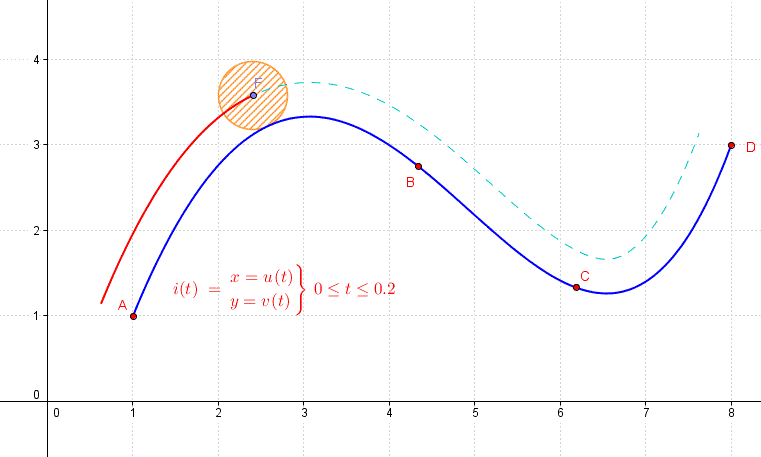
\includegraphics[scale=0.7]{imagens/FiguraTeste.png}
  	\vspace{-12pt}
  	\center {Fonte: Elaborada pelo autor}
  	\label{fig:FiguraTeste}
\end{figure}

De acordo com a figura 1, ...texto ...texto ...texto ...texto ...texto ...texto ...texto ...texto ...texto ...texto ...texto ...texto ...texto ...texto ...texto ...texto ...texto ...texto ...texto ...texto...texto ...texto ...texto ...texto

A Tabela 1 evidencia os dados...

\begin{table}[h]
	\centering
	\caption{Distância percorrida no intervalo 	de tempo entre 4 e 5 segundos}
	\begin{tabular}{c|c|c|c|c|c|c}
	\hline
	Intervalo de tempo (s) & 4,0 & 4,2 & 4,4  & 4,6 & 4,8 & 5,0 \\ \hline
	Distância (m) & 10,0 & 11,02 & 12,16  & 	13,45 & 14,96 & 16,80 \\  \hline  % não é preciso 	quebrar a última linha
	\end{tabular}
	\vspace{-10pt}
	\center {Fonte: Stewart (2012)}
\end{table}

A Equação \ref{eq1} mostra...%não dar enter
\begin{equation}\label{eq1}
P(t)={n \choose i}(1-t)^{n-i} t^i
\end{equation}


Detalhes adicionais sobre a como mencionar as figuras, as tabelas e as equações, o(a) candidato(a) deve consultar a norma NBR 14724.


  % Capitulo 3: Terceiro capítulo (arquivo capitulos/capitulo3.tex)
  % Capítulo 3
\chapter{Capítulo 3}

Algumas regras devem ser observadas na redação da monografia:
\begin{enumerate}
	\item ser claro, preciso, direto, objetivo e conciso, utilizando frases curtas e evitando ordens inversas desnecessárias;
	\item construir períodos com no máximo duas ou três linhas, bem como parágrafos com cinco linhas cheias, em média, e no máximo oito (ou seja, não construir parágrafos e períodos muito longos, pois isso cansa o(s) leitor(es) e pode fazer com que ele(s) percam a linha de raciocínio desenvolvida);
	\item a simplicidade deve ser condição essencial do texto; a simplicidade do texto não implica necessariamente repetição de formas e frases desgastadas, uso exagerado de voz passiva (como \textit{será iniciado}, \textit{será realizado}), pobreza vocabular etc. Com palavras conhecidas de todos, é possível escrever de maneira original e criativa e produzir frases elegantes, variadas, fluentes e bem alinhavadas;
	\item adotar como norma a ordem direta, por ser aquela que conduz mais facilmente o leitor à essência do texto, dispensando detalhes irrelevantes e indo diretamente ao que interessa, sem rodeios (verborragias);
	\item não começar períodos ou parágrafos seguidos com a mesma palavra, nem usar repetidamente a mesma estrutura de frase;
	\item desprezar as longas descrições e relatar o fato no menor número possível de palavras;
	\item recorrer aos termos técnicos somente quando absolutamente indispensáveis e nesse caso colocar o seu significado entre parênteses (ou seja, não se deve admitir que todos os que lerão o trabalho já dispõem de algum conhecimento desenvolvido no mesmo);
	\item dispensar palavras e formas empoladas ou rebuscadas, que tentem transmitir ao leitor mera idéia de erudição;
	\item não perder de vista o universo vocabular do leitor, adotando a seguinte regra prática: \textit{nunca escrever o que não se diria};
	\item termos coloquiais ou de gíria devem ser usados com \textit{extrema} parcimônia (ou mesmo nem serem utilizados) e apenas em casos muito especiais, para não darem ao leitor a idéia de vulgaridade e descaracterizar o trabalho;
	\item ser rigoroso na escolha das palavras do texto, desconfiando dos sinônimos perfeitos ou de termos que sirvam para todas as ocasiões; em geral, há uma palavra para definir uma situação;
	\item encadear o assunto de maneira suave e harmoniosa, evitando a criação de um texto onde os parágrafos se sucedem uns aos outros como compartimentos estanques, sem nenhuma fluência entre si;
	\item ter um extremo cuidado durante a redação do texto, principalmente com relação às regras gramaticais e ortográficas da língua; geralmente todo o texto é escrito na forma impessoal do verbo, não se utilizando, portanto, de termos em primeira pessoa, seja do plural ou do singular.
\end{enumerate}


\section{Seção 1}

Teste de uma tabela:

\begin{table}[htb]
	% Título de tabelas sempre aparecem antes da tabela
	\textsf{\caption{Tabela sem sentido}}
	\center
	{
		\begin{tabular}{l|l}
			\hline
			Titulo Coluna 1   & Título Coluna 2\\
			\hline
			X                 & Y\\
			X                 & W\\
			\hline
		\end{tabular}
	}
	\label{tab:TabelaSemSentido}
\end{table}


\section{Seção 2}

Seção 2


\subsection{Subseção 2.1}

Referência à tabela definida no início: \ref{tab:TabelaSemSentido}


\subsection{Subseção 2.2}

Subsection 2.2


\section{Seção 3}

Seção 3

  % Capitulo 4: Quarto capítulo (arquivo capitulos/capitulo4.tex)
  % Capítulo 4
\chapter{Capítulo 4}

\section{Seção 1}

Teste para símbolo

$\lambda$
%\simb[$\lambda$ (algum símbolo)]{$\lambda$}


\section{Seção 2}

Teste para abreviatura 

\abrv[UFRN -- Universidade Federal do Rio Grande do Norte]{UFRN}

\abrv[DIMAp -- Departamento de Informática e Matemática Aplicada]{DIMAp}


  % Capitulo 5: Quinto capítulo (arquivo capitulos/capitulo5.tex)
  % Capítulo 5
\chapter{Capítulo 5}

\section{Exemplo de algoritmo}

O Algoritmo \ref{alg:howto} usa o pacote {\texttt algorithm2e} que suporta comandos em Português.

\begin{algorithm}[H]
    \SetAlgoLined
    \Entrada{Entrada do algoritmo}
    \Saida{Saída do Algoritmo}
    \Inicio{
        inicialização\;
        \Enqto{condição}{
        instrução\;
        \eSe{condição}{
            instrução1\;
            instrução2\;
        }{
            instrução3\;
        }
        }
        \Para{i de 1 até 10}{
        instrução\;
        }
    }
    \caption{Como escrever algoritmos}
    \label{alg:howto}
\end{algorithm}


\section{Seção 2}

Alguns exemplos de citação: 

Na tese de Doutorado de Paquete \cite{PaquetePhD}, discute-se sobre algoritmos de busca local estocásticos aplicados a problemas de Otimização Combinatória considerando múltiplos objetivos. Por sua vez, o trabalho de \cite{KnowlesBoundedLebesgue}, publicado nos anais do IEEE CEC de 2003, mostra uma técnica de arquivamento também empregada no desenvolvimento de algoritmos evolucionários multi-objetivo, trabalho esse posteriormente estendido para um capítulo de livro dos mesmos autores \cite{KnowlesBoundedPareto}. Por fim, no relatório técnico de \citeonline{Jaszkiewicz}, fala-se sobre um algoritmo genético híbrido para problemas multi-critério, enquanto no artigo de jornal de Lopez \textit{et al.} \cite{LopezPaqueteStu} trata-se do \textit{trade-off} entre algoritmos genéticos e metodologias de busca local, também aplicados no contexto multi-critério e relacionado de alguma forma ao trabalho de Jaszkiewicz (\citeyear{Jaszkiewicz}).

Outros exemplos relacionados encontram-se em \cite{Silberschatz} (livro), \cite{DB2XML} (referência da Web) e \cite{Angelo} (dissertação de Mestrado).

\subsection{Subseção 5.1}

Subseção 5.1

\subsection{Subseção 5.2}

Subsection 5.2

\section{Seção 3}

Seção 3

  % Consideracoes finais
  % Considerações finais
\chapter{Considerações finais}

As considerações finais formam a parte final (fechamento) do texto, sendo dito de forma resumida (1) o que foi desenvolvido no presente trabalho e quais os resultados do mesmo, (2) o que se pôde concluir após o desenvolvimento bem como as principais contribuições do trabalho, e (3) perspectivas para o desenvolvimento de trabalhos futuros. O texto referente às considerações finais do autor deve salientar a extensão e os resultados da contribuição do trabalho e os argumentos utilizados estar baseados em dados comprovados e fundamentados nos resultados e na discussão do texto, contendo deduções lógicas correspondentes
aos objetivos do trabalho, propostos inicialmente.

  \postextual
  
  % Bibliografia (arquivo capitulos/referencias.bib)
  \bibliography{capitulos/referencias}
  % Sistema autor-data
  \bibliographystyle{abntex2-alf}
  % Sistema numérico
  %\bibliographystyle{abntex2-num}

  % Apêndice A (arquivo capitulos/apendices.tex)
  % Apêndice
\begin{apendicesenv}

  \partapendices

  \chapter{Primeiro apêndice}

  Os apêndices são textos ou documentos elaborados pelo autor, a fim de complementar sua argumentação, sem prejuízo da unidade nuclear do trabalho.

\end{apendicesenv}


  % Anexo A (arquivo capitulos/anexos.tex)
  % Anexo
\begin{anexosenv}

  \partanexos

  \chapter{Primeiro anexo}

  Os anexos são textos ou documentos não elaborado pelo autor, que servem de fundamentação, comprovação e ilustração.
\end{anexosenv}


  % Página em branco
  \newpage
\end{document}
